\documentclass{article}
\usepackage[preprint]{nips_2018}
\usepackage[utf8]{inputenc} % allow utf-8 input
\usepackage[T1]{fontenc}    % use 8-bit T1 fonts
\usepackage{hyperref}       % hyperlinks
\usepackage{url}            % simple URL typesetting
\usepackage{booktabs}       % professional-quality tables
\usepackage{amsfonts}       % blackboard math symbols
\usepackage{nicefrac}       % compact symbols for 1/2, etc.
\usepackage{microtype}      % microtypography
\usepackage{packages}
\newcommand{\pfrac}[2]{\frac{\partial #1}{\partial #2}}

\title{Deep Learning Assignment 2}

\author{%
  Jochem Loedeman \\
  12995282
}

\begin{document}
\maketitle
\section{Recurrent Neural Networks}
\subsection{Vanilla RNNs}
\subsubsection*{Question 1.1}
\begin{enumerate}[label=(\alph*)]
	\item
	$$\pfrac{\mathcal{L}^{(T)}}{\b W_{ph}} = \pfrac{\mathcal{L}^{(T)}}{\b p^{(T)}}\pfrac{\b p^{(T)}}{\b W_{ph}}$$ In the computational graph, there is no path from outputs of recurrent hidden states to the loss at $T$. Therefore, no sum over previous states is present in the expression for the gradient.
	\item
	$$
	\begin{aligned}
	\pfrac{\mathcal{L}^{(T)}}{\b W_{hh}} &= \pfrac{\mathcal{L}^{(T)}}{\b p^{(T)}}\pfrac{\b p^{(T)}}{\b h^{(T)}}\pfrac{\b h^{(T)}}{\b W_{hh}} = \sum_{i=0}^{T}\pfrac{\mathcal{L}^{(T)}}{\b p^{(T)}}\pfrac{\b p^{(T)}}{\b h^{(T)}}\pfrac{\b h^{(T)}}{\b h^{(i)}}\pfrac{\b h^{(i)}}{\b W_{hh}} \\ &= \sum_{i=0}^{T}\pfrac{\mathcal{L}^{(T)}}{\b p^{(T)}}\pfrac{\b p^{(T)}}{\b h^{(T)}}\left(\prod_{j=i+1}^T\pfrac{\b h^{(j)}}{\b h^{(j-1)}}\right)\pfrac{\b h^{(i)}}{\b W_{hh}}
	\end{aligned}
	$$ In this case, there are paths from nodes in previous timesteps computed with $\b W_{hh}$ to the loss at $T$. Therefore, we should account for these dependencies through the chain rule, giving rise to sums and products within the expression for the gradient.
	\item The first and second gradients are respectively independent and dependent on previous timesteps, as was already explained through the connectivity of the computational graph. When training this network for a large number of timesteps, we have to account for very long-term dependencies of the recurrent states through the product in the expression for the second gradient. This product of Jacobians can cause the total gradient to become very small or very large, making learning difficult.
\end{enumerate}
\subsection{Long Short-Term Memory (LSTM) network}
\subsubsection*{Question 1.2}
\begin{enumerate}[label=(\alph*)]
	\item
	\begin{itemize}
		\item \textit{Input modulation gate:} \\Proposes an updated cell state. This gate has a tanh activation, which is important to keep the activations of the internal state zero-centered. If for example we used the sigmoid, these states would increase over time. \\
		\item \textit{Input gate:}\\ Regulates how much of the new value proposed by the input modulation gate is actually used in the updated cell state. Uses a sigmoid to obtain a gating value between 0 and 1.\\
		\item \textit{Forget gate:}\\ Regulates how much of the previous cell state is retained in the updated cell state. Uses a sigmoid to obtain a gating value between 0 and 1, which corresponds to completely forgetting or strongly remembering the previous state. \\
		\item \textit{Output gate:}\\ Regulates how much of the nonlinearized current cell state is passed as output of the cell. Uses a sigmoid to obtain a gating value between 0 and 1.\\
	\end{itemize}
	\item 
	$$
	\begin{aligned}
	N_{\text{total}} = 4&\underbrace{\left(N_{\text{hidden}}\cdot N_{\text{input}} + N_{\text{hidden}}\cdot N_{\text{hidden}} + N_{\text{hidden}}\right)}_{\text{gate input weights, recurrent weights and biases}} \\ &+ \underbrace{N_{\text{output}}\cdot N_{\text{hidden}}}_{\text{output weights}} + \underbrace{N_{\text{output}}}_{\text{output bias}}
	\end{aligned}
	$$
\end{enumerate}
\subsection{LSTMs in PyTorch}
\subsubsection*{Question 1.3}
The required LSTM model was implemented in PyTorch, and evaluated using the supplied \texttt{train} function and the binary palindrome data. Accuracies were obtained for sequence lengths of 10 and 20, where each hyperparameter setting was evaluated for 3 different random seeds (0, 1 and 2). From these results, the mean and standard deviation for each accuracy value was obtained. This yielded two accuracy curves, one for each sequence length setting, together with the corresponding standard deviations. They are shown in Figure \ref{fig:lstm}, where the shaded areas correspond to the accuracy values that lie within 1 standard deviation on either side of the obtained accuracy value. Notice that for $T = 20$ the standard deviation increases strongly after $1000$ steps. At this point, some training runs make a large jump in accuracy, whereas others fall behind. This behaviour seems to be characteristic of the model on this data; the accuracy is stable around $0.55$ when suddenly, the model improves relatively quickly to perfect accuracy.
\begin{figure}[h]
	\centering
	\subfloat[]{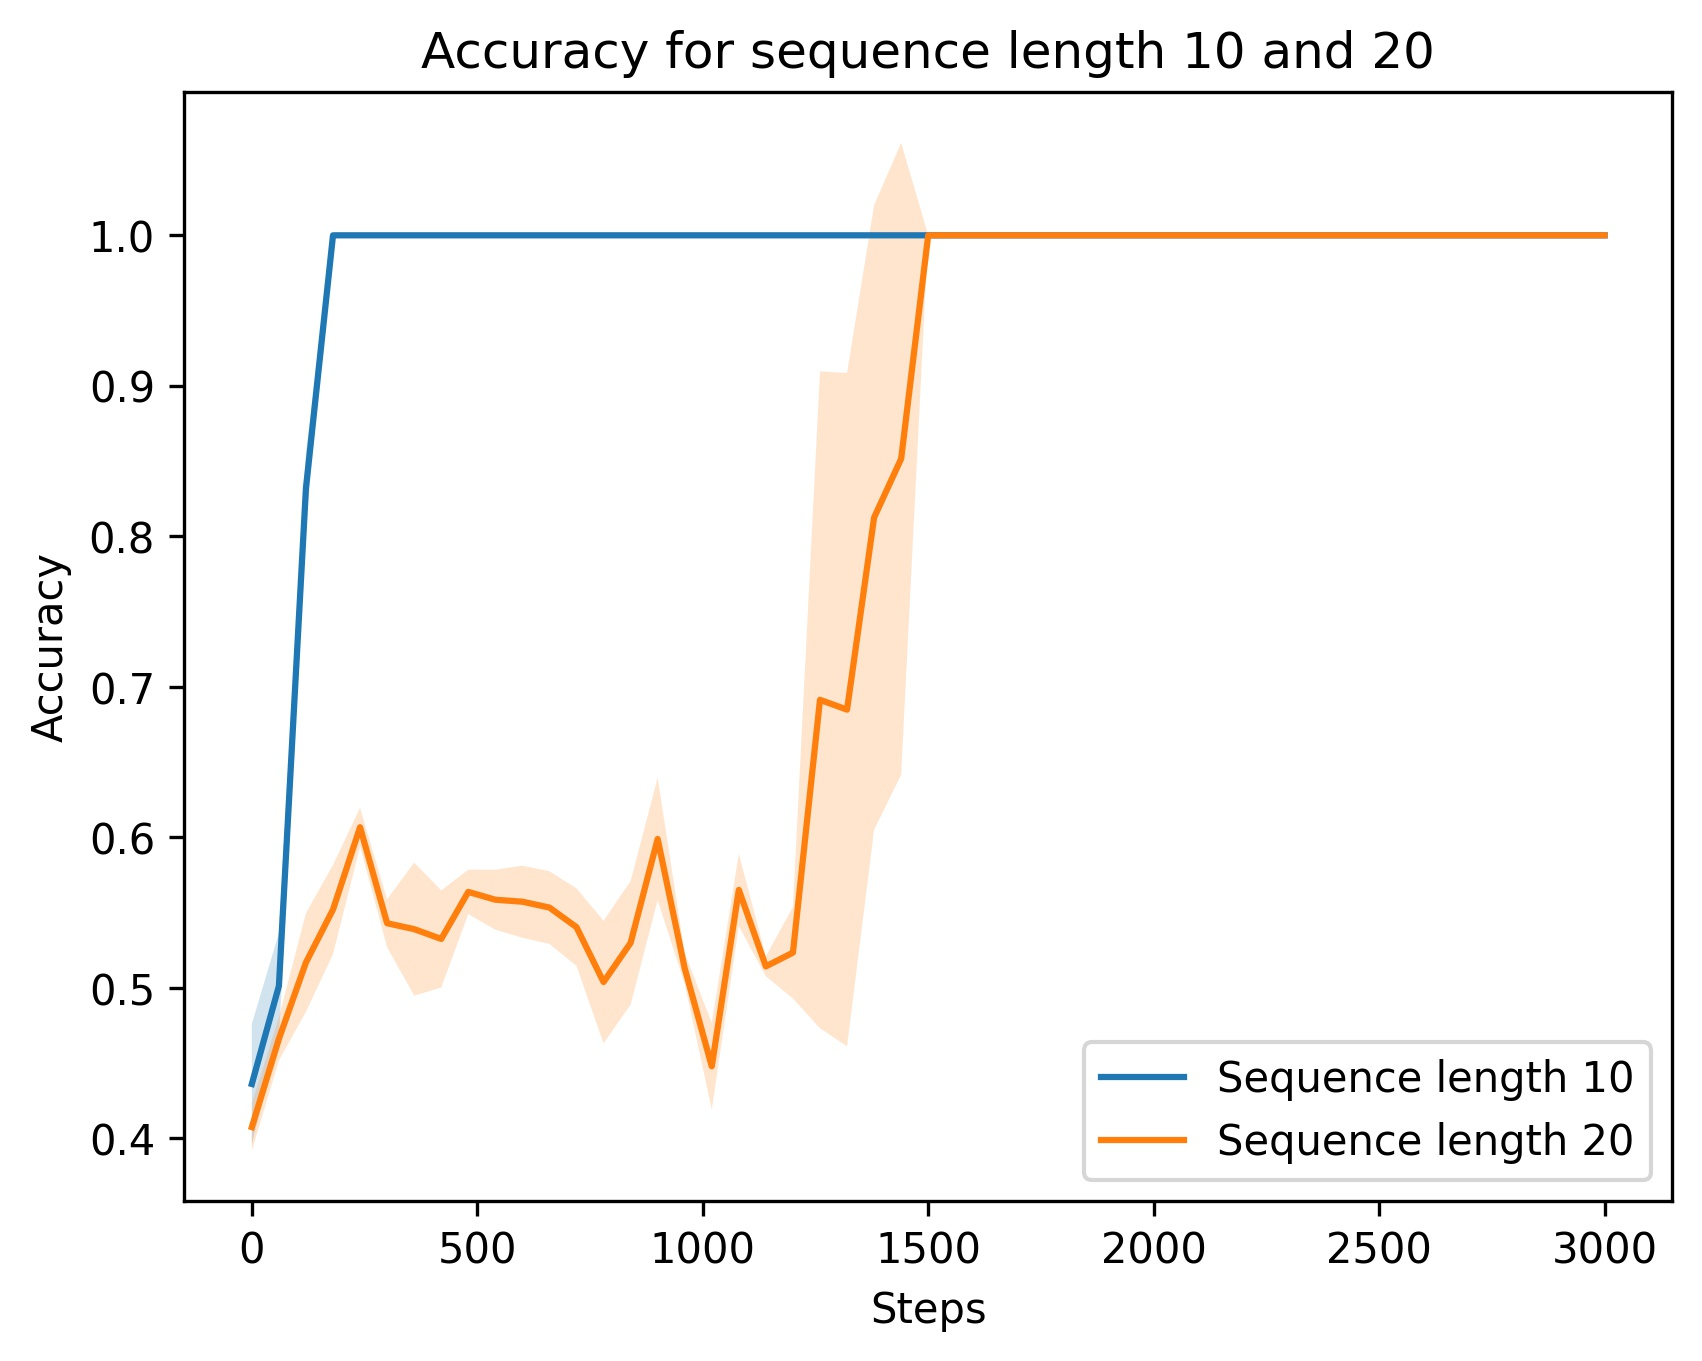
\includegraphics[width=.8\textwidth]{lstm.jpg}}
	\caption{Accuracy of the LSTM on the binary palindrome dataset for $T=10$ and $T = 20$}
	\label{fig:lstm}
\end{figure}
\subsubsection*{Question 1.4}
The peepLSTM model was implemented in PyTorch, using the same hyperparameter settings as before. The results are shown in Figure \ref{fig:peeplstm}. For $T = 20$ the model converges to perfect accuracy already around $500$ steps, which is significantly faster than the original LSTM model. Furthermore, the uncertainty of the accuracy values is much smaller. Apparently, setting the gate values based on the cell states rather than the LSTM outputs is beneficial for the performance of the model on this data set.
\begin{figure}[h]
	\centering
	\subfloat[]{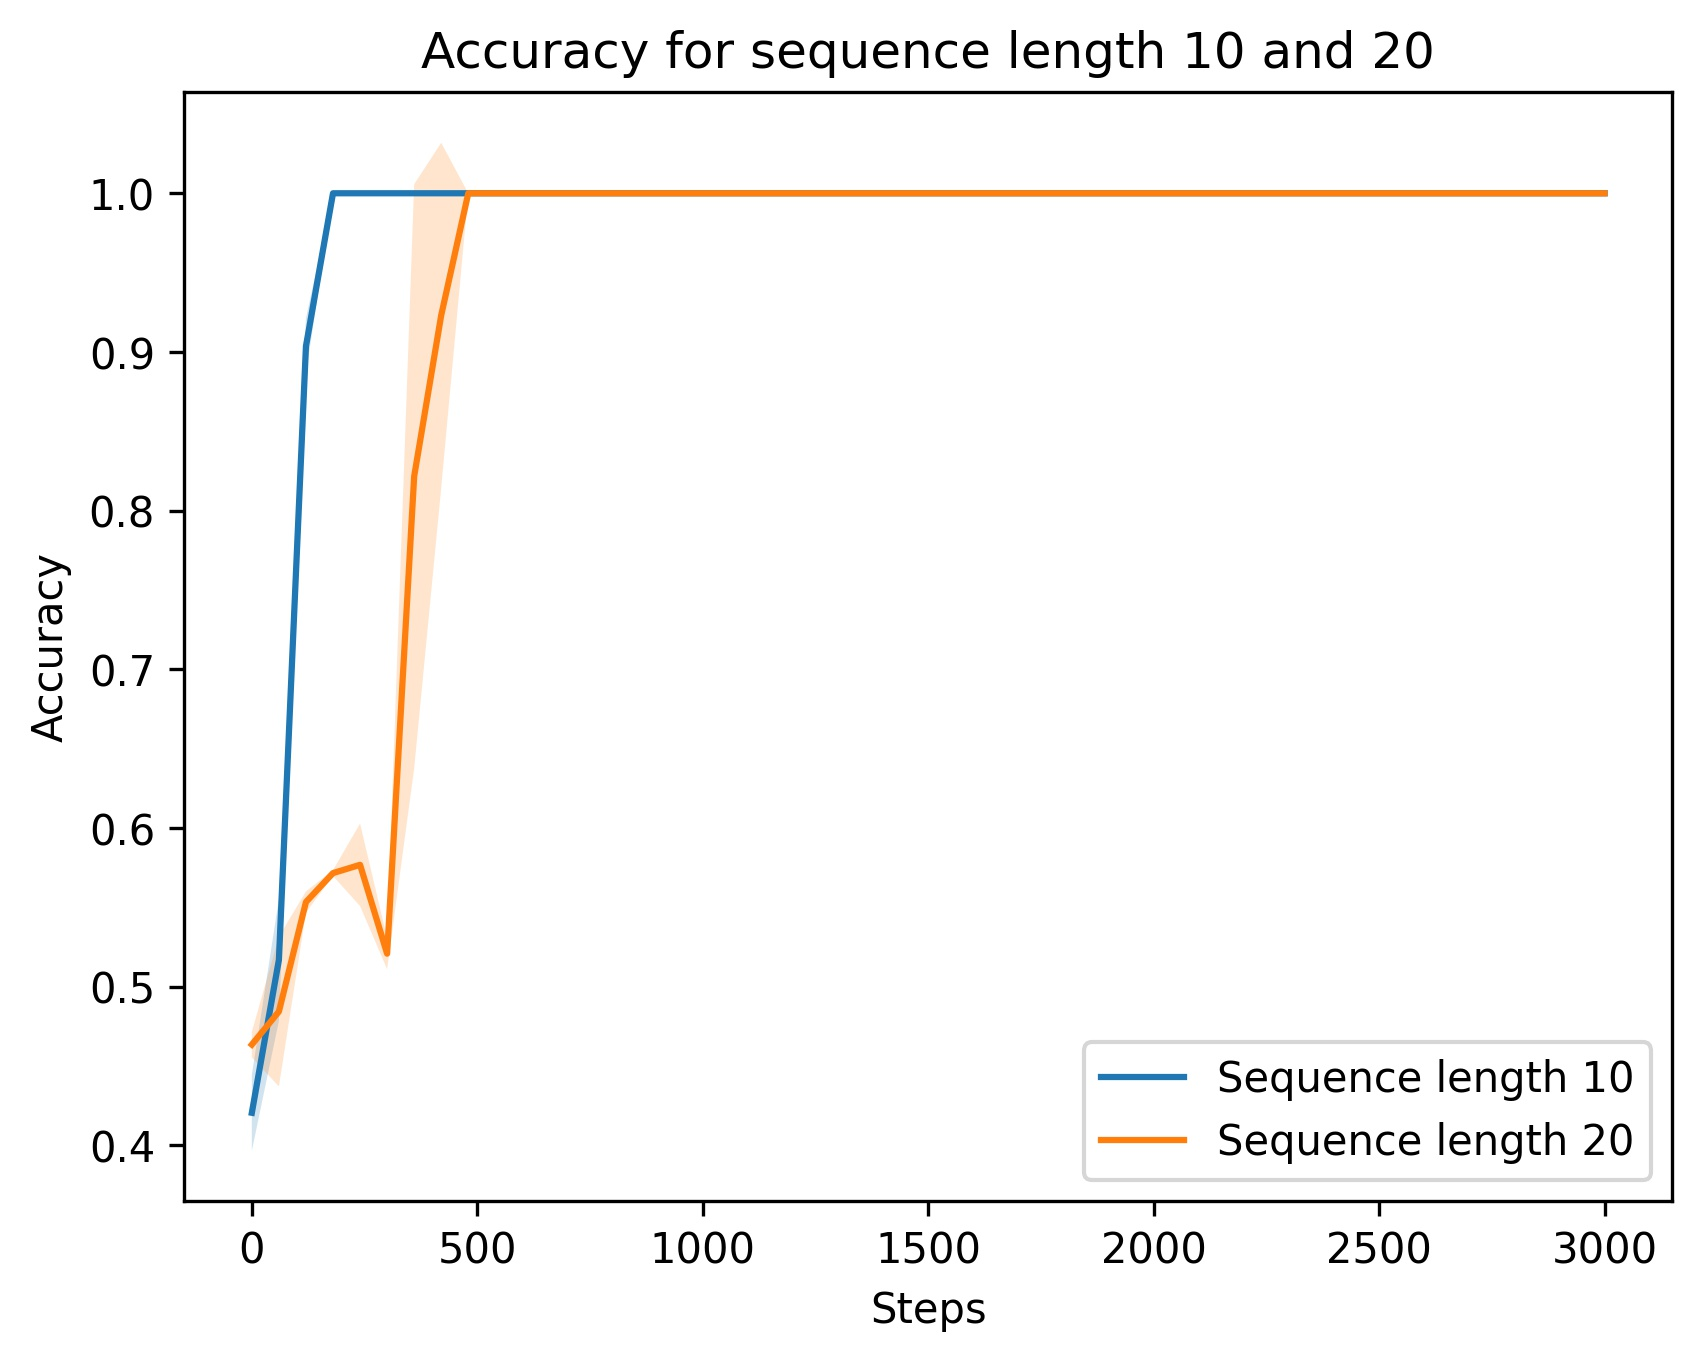
\includegraphics[width=.8\textwidth]{peep_lstm.jpg}}
	\caption{Accuracy of the peepLSTM on the binary palindrome dataset for $T=10$ and $T = 20$}
	\label{fig:peeplstm}
\end{figure}
\section{Recurrent Nets as Generative Model}
\subsubsection*{Question 2.1}
\begin{enumerate}[label = (\alph*)]
	\item 
\end{enumerate}
\end{document}